\section{\tool\ Design}
\label{sec:approach}
%\vspace{-2mm}

\begin{figure}
	\centering
		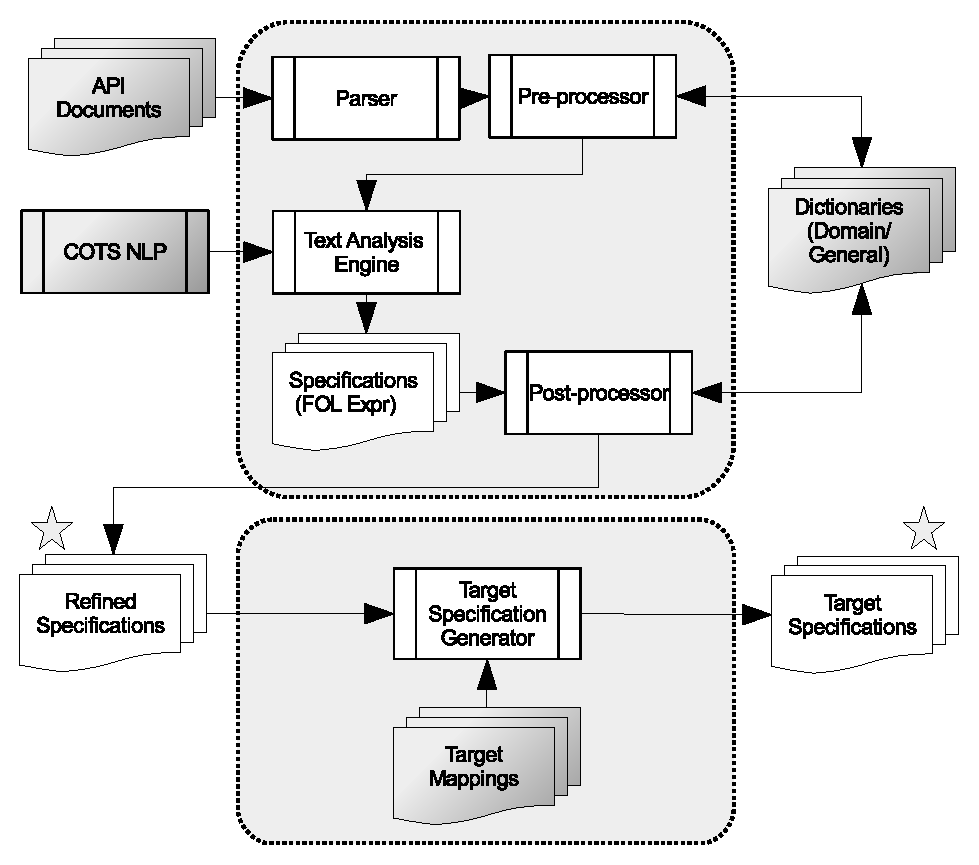
\includegraphics[scale=0.45]{approach.eps}
	\caption{Overview of \tool\ framework}
	\label{fig:approachOverview}
\end{figure}

We next present our framework for inferring specifications from the method descriptions in API Documents. Figure~\ref{fig:approachOverview} gives an overview of our framework. Our framework consists of four major components: a parser, a preprocessor, an text-analysis engine, and a postprocessor.

The parser accepts online API description and parser them into an intermediate representation. The pre-processor accepts method descriptions and preprocesses the sentences in the descriptions, such as annotating sentence boundaries and reducing lexical tokens. 
The text-analysis engine accepts the pre-processed sentences and parses them using an NLP parser. The text-analysis engine further transforms the parsed sentences into the first-order-logic (FOL) representation and then leverages the FOL representation of a sentence to infer specifications. Finally, the postprocessor undoes any modifications done by the preprocessor to get refined specifications.

Besides the previously described major components the framework also consists of a an external component, namely target specification generator. This component accepts the specification generated by our framework and using mapping functions to a target specification language generates specifications in the target language of choice. We next describe each component in detail.


\subsection{Parser}
\label{sub:parser}

Our parser accepts the online API documents and parses them into predefined categories. In particular, our parser extracts the following contents: 1) Summary of the API method, 2)Summary of request elements of the method, and 3) Summary of response elements of the method inclusive of error responses.

This step is required to extract the desired descriptive text from the various presentation styles of the API documents. In particular, deferential API documents may have styles of presenting information to developers inclusive of different levels of details, we chose very generic fields that are found across all documents. 

Currently our prototype implementation extracts this information from \amazon. However almost all of the REST API developer documents are provided on-line as structured webpages, thus the parser can be easily extended to extract desired information from any REST API developer documents in general.    


\subsection{Preprocessor}
\label{sub:Preprocessor}

The preprocessor accepts method application descriptions extracted by the parser and preprocesses the natural language text, to be further analyzed by the text-analysis engine. In particular, the preprocessor annotates special words and reduces the number of lexical tokens using semantic information. The preprocessing steps are required to increase the accuracy of the subsequent phases of \tool\ framework, described in detail in Section~\ref{sub:TAE}. We next describe in detail the preprocessing steps:

\textbf{1. Special word annotation}.
Since the exiting NLP techniques rely on accurate annotation of POS tags in a sentence, the accuracy of \tool\ to infer constraints is dependent on the accurate annotation of POS tags. While existing techniques work well on general linguistics, that does not necessary entail that they work well with domain specific text as well. In particular, with respect to API documents certain words have a very different semantic meaning, in contrast to general linguistics that causes incorrect annotation of POS tags.

Consider the word ``POST'' for instance. The online Oxford dictionary~\footnote{\url{http://oxforddictionaries.com/us/definition/american_english/post?q=POST}} has 8 different definition of word ``POST'', and none of them describes POST as a HTTP method supported by REST API meaning: \textit{``Creates a new entry in the collection. The new entry's URI is assigned automatically and is usually returned by the operation''}. Thus existing NLP techniques fail to accurately annotate the POS tags of the sentences involving word ``POST''.  

This preprocessing step identifies such words from the sentences based on a domain-specific dictionary, and annotates them appropriately. This special annotation forces the underlying POS tagger to accurately annotate the POS tags of the words involving domain specific keywords.

From implementations perspective, we manually built the domain-specific dictionary using the glossary of terms collected from the web pertaining to REST API. We further leveraged the HTML style information in \amazon\ to look for words that were highlighted in code like format. 

\textbf{2. Lexical tokens reduction}.

The reduction of lexical tokens greatly increases the accuracy of the analysis in the subsequent components of our framework. In particular, the preprocessor reduces lexical tokens by performing following subtasks

\textbf{1. Period Handling}. Besides marking the end of a sentence in simplistic English, the character period (`.') has other legal usages as well such as decimal representation (periods between numbers). Although legal, such usage hinder detection of sentence boundaries, thus forcing the subsequent components to return incorrect or imprecise results. We pre-process the sentences by annotating these usages for accurate detection of sentence boundaries. We achieve so by looking up known shorthand words from WordNet~\cite{wordnet} and detecting decimals, which are also the period character, by using regular expressions. From an implementation perspective, we have maintained a static lookup table of shorthand words observed in WordNet.
	
\textbf{2. Named Entity Handling}. Sometimes a sequence of words correspond to the name of entities that have a specific meaning collectively. For instance, consider the phrases \textit{``Amazon S3'', ``Amazon simple storage service''}, which are the names of the service. Further resolution of these phrases using grammatical syntax is unnecessary and would not bring forth any semantic value. Also these phrases contribute to length of a sentence that in turn negatively affects the accuracy of POS tagger. Thus, we identify such phrases and annotate them as single lexical units. We achieve so by maintaining a static lookup table.
	
\textbf{3. Abbreviation Handling}. Natural-language sentences often consist of abbreviations mixed with text. This can result in subsequent components to incorrectly parse a sentence. We find such instances and annotate them as a single entity. For example, text followed by abbreviations such as \textit{``Access Control Lists (ACL)''} is treated as single lexical unit. Detecting such abbreviations is achieved by using the common structure of abbreviations and encoding such structures into regular expressions. Typically, regular expressions provide a reasonable approximation for handling abbreviations. 
	
\textbf{4. Frequent Phrases} Although the previous steps assist in bringing down the number of lexical tokens in a sentence, some sentences may still contain a considerable number of lexical tokens to overwhelm the underlying POS tagger. To address this issue we propose to further reduce the number of lexical tokens in a sentence  by annotating frequent phrases as a single lexical unit.

In particular, we use n-gram based approach as means to achieve this reduction. In the fields of computational linguistics and probability, an n-gram is a contiguous sequence of n words from a given sequence of text or speech. We first calculate the most frequently occurring n-grams in the text body. In particular, we are interested in the n-grams of length 4 or greater to achieve a reasonable reduction. We then prune the list of n-grams based on a subsumption. We consider a n-gram of length k ($n_k$) to subsume n-gram of length k-1 ($n_{k-1}$) iff $n_{k-1}$ is a substring of ($n_k$) and the frequency of occurrence of $n_{k-1}$ equals frequency of occurrence of $n_{k}$ . Finally, we rank the list of n-grams based on the frequency of their occurrence in the text, and select top-k n-grams for reduction.
 
From an implementation perspective we used Apache Lucene$^{\textregistered}$~\cite{lucene} to achieve n-gram reduction. Apache Lucene is a high-performance, full-featured text search engine library written entirely in Java. It is a technology suitable for nearly any application that requires full-text search, especially cross-platform.

Although a POS tagger can be retrained to achieve these pre-processing steps, we prefer annotations to make our approach independent of any specific NLP infrastructure, thus ensuring interoperability with various POS taggers.
	
\subsection{NLP Parser}


The NLP parser accepts the pre-processed documents and annotates every sentence within each document using standard NLP techniques. From an implementation perspective, we chose the Stanford Parser~\cite{SNLP}. However, this component can be implemented using any other existing NLP libraries or frameworks. In particular, we annotate each sentence with POS annotations, Named-Entity Annotations and Stanford-Typed Dependencies. For more details on these tehniques and their application, please refer to ~\cite{Marneffe06LREC,Marneffe08COLING,pandita12:inferring, pandita13:WHYPER}.

%\begin{figure}
%	\centering
%%		\includegraphics[scale=0.6]{stanfordAnnotated.eps}
%	\caption{Sentence annotated with Stanford dependencies}
%	\label{fig:standep}
%\end{figure}
%
%Next we use an example to illustrate the annotations added by the NLP Parser. Consider the example sentence \textbf{\textit{``Also you can share the yoga exercise to your friends via Email and SMS.''}}, that indirectly refers to the READ\_CONTACTS permission. Figure~\ref{fig:standep} shows the sentence annotated with Stanford-typed dependencies. The words in red are the names of dependencies connecting the actual words of the sentence (in black). Each word is followed by the Part-Of-Speech (POS) tag of the word (in green). For more details on Stanford-typed dependencies and POS tags, please refer to ~\cite{Marneffe06LREC,Marneffe08COLING}.




\subsection{Text Analysis Engine}
\label{sub:TAE}
%
%\begin{figure}
%	\centering
%	%	\includegraphics[scale=0.65]{taeRep.eps}
%	\caption{First-order logic representation of annotated sentence in Figure~\ref{fig:standep}}
%	\label{fig:FOLRep}
%\end{figure}

The text analysis engine component accepts the annotated documents and creates an intermediate representation of each sentence. We define our representation as a tree structure that is essentially a First-Order-Logic (FOL) expression. Research literature provides evidence of the the adequacy of using FOL for NLP related analysis tasks~\cite{Sinha2009,Sinha2010,pandita12:inferring, pandita13:WHYPER}.

In our representation, every node in the tree except for the leaf nodes is a predicate node. The leaf nodes represent the entities. The children of the predicate nodes are the participating entities in the relationship represented by the predicate. The first or the only child of a predicate node is the governing entity and the second child is the dependent entity. Together the governing entity, predicate and the dependent entity node form a tuple.  


In particular, the process of generation of intermediate-representation is an extension of the intermediate-representation generator component of \emph{WHYPER}~\cite{pandita13:WHYPER} with additional steps. In \emph{WHYPER}, the intermediate representation is generated based on principle of shallow parsing~\cite{Branimir2000}. They implemented their parser as a function of Stanford-typed dependencies~\cite{Marneffe06LREC,Marneffe08COLING,SNLP,KleinNIPS03}, to leverage the semantic information encoded in Stanford-typed dependencies.

However, we observed that intermediate-representation generator component of \emph{WHYPER}~\cite{pandita13:WHYPER} is overwhelmed by wordy sentences.This limitation mandates the use of additional novel technique of \textit{`Frequent Phrases Reduction'} in preprocessing phase. We further improve the accuracy of  parser by adopting a hybrid (leveraging both POS tags as well as Stanford-typed dependencies) approach.

Our implementation of shallow parser is a two phase process:

\begin{enumerate}
	\item{\textbf{POS Tags}}: We first parse a sentence based on the function of POS tags. In particular, we use semantic templates to logically break a sentences into smaller constituent sentences. For instance, consider the sentence \scriptsize``All objects (including all object versions and Delete Markers) in the bucket must be deleted before the bucket itself can be deleted.''. \normalsize The Stanford parser inaccurately annotates the Stanford-typed dependencies of the sentence because of presence of different clauses acting on different subject-object pairs. We thus break down the sentence into two smaller tractable sentences:
	
	 \scriptsize All objects in the bucket must be deleted before the bucket itself can be deleted.
	
	 All objects including all object versions and Delete Markers.\normalsize 
	 
	 Table~\ref{tab:semanticTemplates} shows a list the semantic templates. Column ``Template'' describes conditions where the template is applicable and Column ``Summary'' describes the action taken by our shallow parser when the template is applicable. All of these semantic templates are publicly available on our project website~\cite{projectweb}. With respect to the previous example the template no. 3 \textit{( A noun phrase followed by another noun/pronoun/verb phrase in brackets)} is applicable. Thus our shallow parser breaks the sentence into two individual sentences.
	 
	\item{\textbf{Stanford-typed Dependencies}}: This phase is equivalent to the intermediate-representation generator component of the \emph{WHYPER}~\cite{pandita13:WHYPER}.

\end{enumerate}

\begin{table*}
\begin{center}

\caption{Semantic Templates}
    \begin{tabular}{ | l | p{5cm} |p{10cm} |}
    \hline
    \textbf{S No.} 	& \textbf{Template} & \textbf{Summary} \\ \hline
    
    1. 		& Two sentences joined by a conjunction & Sentence is broken down into two individual sentences with the conjunction term serving as the connector between two. \\ \hline
    2. 		& Two sentences joined by a ``,''& Sentence is broken down to individual independent sentences \\ \hline
    3.		& A noun phrase followed by another noun/pronoun/verb phrase in brackets & Two individual sentences are formed. The first sentence is  the same as the parent sentence sans the noun/pronoun.verb phrase in bracket. The second sentence constitutes of the noun phrase followed by  noun/pronoun/verb phrase without the brackets.\\ \hline
    4.		& A noun phrase by a conditional phrase in brackets & Two individual sentences are formed. The first sentence is the same as the parent sentence sans the conditional phrase in bracket. The second sentence constitutes of noun phrases followed by conditional in the bracket.\\ \hline
    5.		& A conditional phrase followed by a sentence & Two dependent sentences are formed. The first sentence constitutes the conditional phrase. The second sentence constitutes rest of the sentence.\\ \hline
    6.		& A sentence in which the parent verb phrase is over two child verb phrases joined by a conjunction & Two dependent sentences are formed where the dependency is the conjunction. The first sentence is formulated by removing conjunction and second child verb phrase. The second sentence is formulated by removing conjunction and first child verb phrase. \\ \hline
    \end{tabular}
	\label{tab:semanticTemplates}
\end{center}
\end{table*}







%The FOL representation helps us effectively deal with the problem of \emph{confounding effects} of keywords as described in Section~\ref{sec:overview}. In particular, the FOL assists in distinguishing between a resource that would be a leaf node and an action that would be a predicate node in the intermediate representation of a sentence. The generated FOL representation of the sentence is then provided as an input to the semantic engine for further processing.
%
%
%
%\subsection{Semantic Engine (SE)}
%\label{sub:SE}
%The Semantic Engine (SE) accepts the FOL representation of a sentence and based on the semantic graphs of Android permissions annotates a sentence if it matches the criteria. A semantic graph is basically a semantic representation of the resources which are governed by a permission. For instance, the READ\_CONTACTS permission governs the resource ``CONTACTS'' in Android system.
%
%
%Figure~\ref{fig:knowledge} shows the semantic graph for the permission READ\_CONTACTS. A semantic graph primarily constitutes of subordinate resources of a permission (represented in rectangular boxes) and a set of available actions on the resource itself (represented in curved boxes). Section~\ref{sub:ACA} elaborates on how we build such graphs systematically.
%
%Our SE accepts the semantic graph pertaining to a permission and annotates a sentence based on the algorithm shown in Algorithm~\ref{alg:SenAnnotaator}. The Algorithm accepts the FOL representation of a sentence $rep$, the semantic graph associated with the resource of a permission $g$ and a boolean value $recursion$ that governs the recursion. The algorithm outputs a boolean value $isPStmt$, which is \CodeIn{true} if the statement describes the permission associated with a semantic graph ($g$), otherwise \CodeIn{false}. 
%
%Our algorithm systematically explores the FOL representation of the sentence to determine if a sentence describes the need for a permission. First, our algorithm attempts to locate the occurrence of associated resource name within the leaf node of the FOL representation of the sentence (Line 3). The method \CodeIn{findLeafContaining(name)} explores the FOL representation to find a leaf node that contains term \CodeIn{name}. Furthermore, we use WordNet and Lemmatisation~\cite{Do09:Robust} to deal with synonyms of a word in question to find appropriate matches. Once a leaf node is found, we systematically traverse the tree from the leaf node to the root, matching all parent predicates as well as immediate child predicates [Lines 5-16].
%
%Our algorithm matches each of the traversed predicate with the actions associated with the resource defined in semantic graph. Similar to matching entities, we also employ WordNet and Lemmatisation~\cite{Do09:Robust} to deal with synonyms to find appropriate matches. If a match is found, then the value \CodeIn{isPStmt} is set to  \CodeIn{true}, indicating that the statement describes a permission.
%
%In case no match is found, our algorithms recursively search all the associated subordinate resources in the semantic graph of current resource. A subordinate resource may further have its own subordinate resources. Currently, our algorithm considers only immediate subordinate resources of a resource to limit the false positives.
%
%%We limit the exploration to depth 1 to limit the false positives. That means only immediate subordinate resources of a resource will be explored.
%
%In the context of the FOL representation shown in Figure~\ref{fig:FOLRep}, we invoke Algorithm~\ref{alg:SenAnnotaator} with the semantic graph shown in Figure~\ref{fig:knowledge}. Our algorithm attempts to find a leaf node containing term ``CONTACT'' or some of its synonym. Since the FOL representation does not contain such a leaf node, algorithm calls itself with semantic graphs of subordinate resources (Line 17-25), namely `NUMBER', `EMAIL', `LOCATION', `BIRTHDAY', `ANNIVERSARY'. 
%
%The subsequent invocation will find the leaf-node ``email'' (annotated 9 in Figure~\ref{fig:FOLRep}). Our algorithm then explores the preceding predicates and finds predicate ``share'' (annotated 2 in Figure~\ref{fig:FOLRep}). The Algorithm matches the word ``share'' with action ``send'' (using Lemmatisation and WordNet similarity), one of the actions available in the semantic graph of resource `EMAIL' and returns \CodeIn{true}. Thus, the sentence is appropriately identified as describing the need for permission READ\_CONTACT. 
%
%
%\algsetup{indent=1em}
%\begin{algorithm}[t!]
%\begin{algorithmic}[1]
%\begin{scriptsize}
%\REQUIRE K\_Graph $g$, FOL\_rep $rep$, Boolean $recursion$ 
%\ENSURE Boolean $isPStmt$
%\STATE $Boolean\ isPStmt\ =\ false$
%\STATE $String\ r\_name\ =\ g.resource\_Name$
%\STATE $FOL\_rep\ r'\ =\ rep.findLeafContaining(r\_name)$
%\STATE $List\ actionList\ =\ g.actionList$
%\WHILE{$(r'.hasParent)$}
%	\IF{$actionList.contains(r'.parent.predicate)$}
%		\STATE $isPStmt\ =\ true$
%		\STATE $break$
%	\ELSE
%		\IF{$actionList.contains(r'.leftSibling.predicate)$}
%			\STATE $isPStmt\ =\ true$
%			\STATE $break$
%		\ENDIF
%	\ENDIF
%	\STATE $r'\ =\ r'.parent$
%\ENDWHILE
%\IF{$((NOT(isPStmt))\ AND\ recursion)$}
%	\STATE $List\ resourceList\ =\ g.resourceList$
%	\FORALL{$(Resource\ res\ in\ resourceList)$}
%		\STATE $isPStmt\ =\ Sentence\_Annotator(getKGraph(res),\ rep,\ false)$
%		\IF{$isPStmt$}
%			\STATE $break$
%		\ENDIF
%	\ENDFOR
%\ENDIF
%\RETURN $isPStmt$
%\end{scriptsize}
%\end{algorithmic}
%\caption{Sentence\_Annotator}
%\label{alg:SenAnnotaator}
%\end{algorithm} 
%
%\begin{figure}
%	\centering
%%		\includegraphics[scale=0.4]{knowledge.eps}
%	\caption{Semantic Graph for the READ\_CONTACT permission}
%	\label{fig:knowledge}
%\end{figure} 
%  
%
%
